\chapter{Utilizzo}
\section{Navigazione}
Appena aperta, l'applicazione mostrerà la seguente schermata:
\begin{figure}[H]
	\centering
	\caption[La pagina iniziale]{La pagina che è mostrata appena l'applicazione è aperta}
	\label{fig:landing-page}
	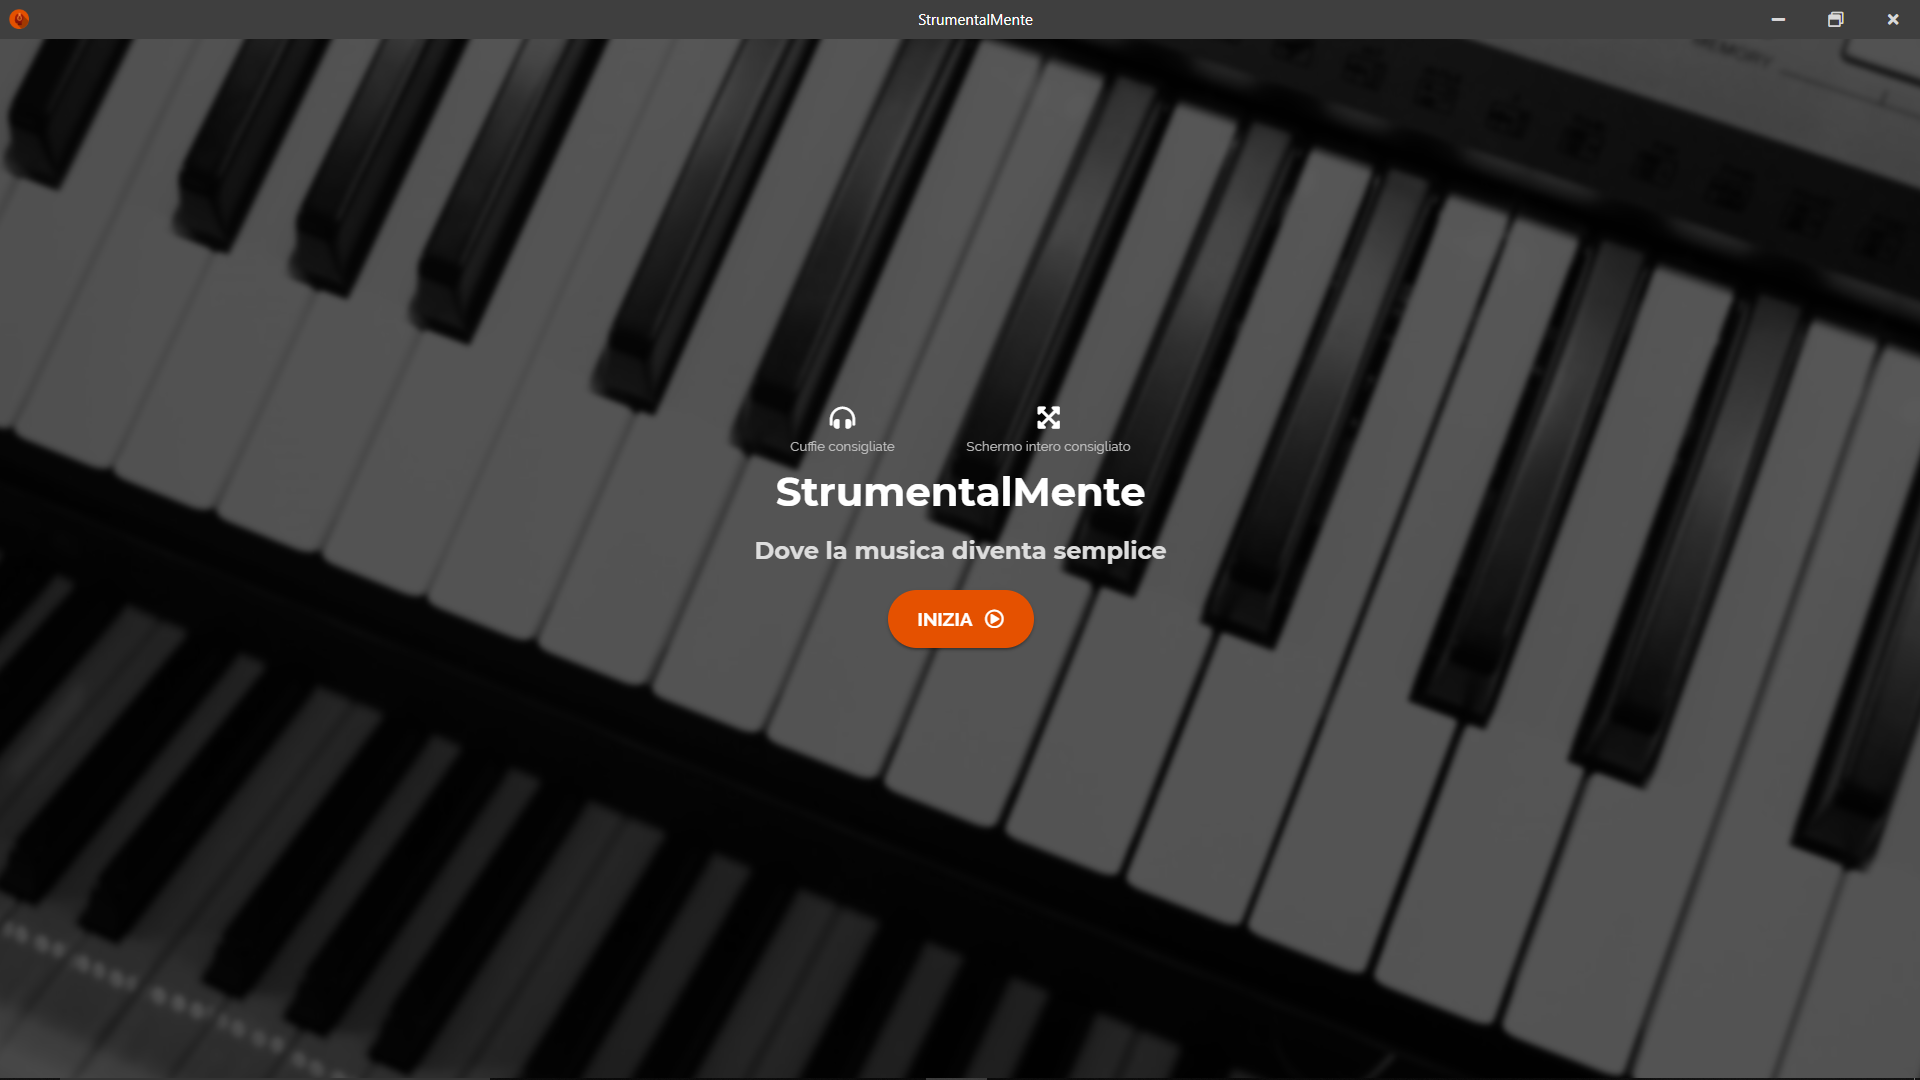
\includegraphics[width=\textwidth]{images/landing-page}
\end{figure}
Per entrare nell'applicazione basta cliccare sul tasto "inizia". Si noti che è possibile procedere semplicemente cliccando il tasto "Invio" ("\textit{Enter}") sulla tastiera. Per maggiori informazioni su ulteriori scorciatoie da tastiera, si veda la sezione \ref{sec:shortcuts} a pagina \pageref{sec:shortcuts}.
\paragraph{Note di visualizzazione} Come suggerito in questa pagina, è fortemente consigliato l'uso delle cuffie e la visualizzazione in modalità "massimizzata" (schermo intero).
\section{Scorciatoie da tastiera}\label{sec:shortcuts}